\documentclass[12pt]{article}

\usepackage[utf8]{inputenc}
\usepackage[T1]{fontenc}
\usepackage{graphicx}
\usepackage{amsmath}
\usepackage{amssymb}
\usepackage{fancyhdr}
\usepackage{geometry}
\usepackage{hyperref}
\usepackage{booktabs}
\usepackage{caption}
\usepackage{titlesec}
\usepackage[expansion=false]{microtype}

\geometry{margin=1in}
\emergencystretch=3em
\sloppy
\raggedbottom
\makeatletter
\setlength{\@fptop}{0pt}
\setlength{\@fpbot}{0pt plus 1fil}
\makeatother

\hypersetup{
    colorlinks=true,
    linkcolor=black,
    citecolor=black,
    urlcolor=black
}

\newcommand{\shorttitle}{Reddit Data Collection Pipeline: r/kolkata \& r/KolkataCity}

\pagestyle{fancy}
\fancyhf{}
\renewcommand{\headrulewidth}{0pt}
\renewcommand{\footrulewidth}{0.4pt}
\fancyfoot[L]{\shorttitle}
\fancyfoot[R]{Page \thepage}

\titleformat{\section}{\large\bfseries}{\thesection.}{0.6em}{}
\titleformat{\subsection}{\normalsize\bfseries}{\thesubsection.}{0.6em}{}
\titleformat{\subsubsection}{\normalsize\bfseries}{\thesubsubsection.}{0.6em}{}

\newcommand{\sectionbreak}{\clearpage}

\begin{document}

% ---------------------------------------------------------------
% TITLE PAGE
% ---------------------------------------------------------------
\begin{titlepage}
\centering
\vspace*{1cm}
{\large\bfseries MidSem Report Design Project}\\[0.8cm]
{\Large\bfseries A Resumable, Multi-Source Pipeline for Collecting\\
and Processing Reddit Data from\\
r/kolkata and r/KolkataCity}\\[1.5cm]


\includegraphics[width=4cm]{bits_logo.png}\\[1.5cm]

{\bfseries\large Harshal Shah}\\
(2023A7PS0055H)\\[1.5cm]

{\bfseries Under Guidance of}\\
{\bfseries\large Prof. Dipanjan Chakraborty}\\
(BITS Pilani, Hyderabad Campus)\\[1.5cm]

{Course Number: CS F377}
\vfill
\end{titlepage}

% ---------------------------------------------------------------
% CONTENTS
% ---------------------------------------------------------------
{\small\tableofcontents}
\clearpage

% ---------------------------------------------------------------
% ACKNOWLEDGMENTS
% ---------------------------------------------------------------
\section*{ACKNOWLEDGMENTS}
\addcontentsline{toc}{section}{ACKNOWLEDGMENTS}

I would like to express my sincere gratitude to my project guide, Prof. Dipanjan Chakraborty, for
his guidance and continuous feedback throughout the design and execution of this project. His
inputs on data collection methodology, API design, and reproducible pipeline engineering were
instrumental in shaping the direction of this work.

I would also like to thank the Birla Institute of Technology and Science (BITS), Pilani, Hyderabad
Campus, for providing the academic environment and computational resources necessary to carry
out this data collection and processing exercise.

I am grateful to my peers in the CS F377 course for the discussions on API rate-limiting
strategies and incremental-collection design that helped refine the pipeline presented in this
report, and to the maintainers of Arctic Shift, the open-source successor to Pushshift, for
making a continuously updated, authentication-free archive of Reddit content publicly available.
I would also like to acknowledge the developers of the \texttt{requests}, \texttt{pandas}, and
\texttt{NumPy} libraries, whose tools made it possible to build this pipeline without having to
re-implement basic HTTP, data-wrangling, and numerical primitives from scratch.

Finally, I acknowledge the original authors of the Pushshift Reddit Dataset, Baumgartner et al.
(2020), whose work on large-scale, academically oriented Reddit archiving motivated the
third-party-archive-first design adopted in this project, and without which a project of this
scope would have been considerably harder to execute given the restrictions placed on Reddit's
own public API.

% ---------------------------------------------------------------
% ABSTRACT
% ---------------------------------------------------------------
\section*{ABSTRACT}
\addcontentsline{toc}{section}{ABSTRACT}

Online communities built around a shared city or region, such as r/kolkata and r/KolkataCity on
Reddit, generate a continuous stream of posts and comments that are a valuable but
operationally awkward data source: individually small, collectively enormous, and governed by
API surfaces that change or disappear with little warning. This project builds a reusable,
resumable, and parameterized collection pipeline that assembles a complete dataset of posts,
comments, subreddit metadata, and cross-post links from these two subreddits, covering 1 April
2025 through the present, in a form suitable for later computational social-science analysis.

The pipeline was designed around two data sources: BrightData's commercial Datasets API, the
original plan, and Arctic Shift, a free, authentication-free, continuously updated successor to
Pushshift. BrightData was used initially to collect the first batch of raw data, but it became
unusable partway through the project for two compounding reasons: the free-tier request quota
on the project's BrightData account was exhausted, and independently, the development network
began intermittently blocking \texttt{api.brightdata.com} with TLS-interception failures. Once
the account's usage limit was reached, continuing to rely on BrightData would have required a
paid upgrade with no guarantee the network-level blocking would also be resolved, so the pipeline
was pivoted to Arctic Shift as its sole active source, with the BrightData client retained as
dead-but-working legacy code. Collection state is tracked per \texttt{(subreddit, data\_type, month)} triple in a
CSV ledger, allowing any interrupted run to resume from exactly where it left off without
re-issuing already-successful API calls, and allowing a new subreddit to be added with no code
change. As of this report, the pipeline has collected 91,328 posts and 566,456 comments for
r/kolkata and 13,499 posts and 176,670 comments for r/KolkataCity, spanning 98,855 unique
authors across both subreddits, of whom 11,836 post or comment in both communities.

This report documents the task specification the pipeline was built against, the dual-source
collection methodology and its resumability guarantees, the resulting dataset's validation
statistics, and the practical engineering challenges encountered while collecting at this scale
on an unreliable local network, including an unplanned scope decision to defer comment
collection for a nine-month stretch of r/kolkata once its true size (nearly seven times larger
than originally expected) became apparent.

The remainder of the report is organized as follows. Section~1 introduces the motivation for
building a city-focused Reddit dataset. Section~2 states the aims and scope of this mid-term
phase, as specified by the original task brief. Section~3 reviews the literature and prior art
that motivated the pipeline's design. Section~4 details the dual-source collection methodology,
state tracking, and resumability design. Section~5 presents the resulting dataset's validation
statistics and activity trends. Section~6 documents the practical engineering challenges
encountered. Sections~7 and 8 close with planned future work and concluding remarks, followed
by a supporting appendix and the full reference list.

\clearpage

% ---------------------------------------------------------------
% 1. INTRODUCTION
% ---------------------------------------------------------------
\section{Introduction to City-Focused Reddit Data Collection}

\subsection{Online Communities as a Data Source}
Subreddits organized around a specific city function as an informal, continuously updated
record of local civic discussion, culture, grievances, and events. Unlike a single survey or a
one-time scrape, a subreddit's post and comment history accumulates over years and reflects
real-time community reaction to events as they happen. For a researcher interested in studying
a city's online public sphere, this history is a uniquely rich data source — provided it can be
collected completely, kept up to date, and stored in a form that supports later analysis without
re-querying the source every time a new question is asked.

\subsection{The Practical Difficulty of Reddit Data Collection}
Collecting this kind of data at scale is harder than it first appears. Reddit's own public API has
become increasingly restrictive since 2023, third-party archival tools such as Pushshift have
had to adapt or be replaced, and any pipeline built against a single external API is exposed to
that API changing, rate-limiting, or disappearing mid-project. A robust collection pipeline must
therefore be designed defensively: resumable so an interruption never forces a costly
re-download, parameterized so it is not hand-wired to a single subreddit, and tolerant of a data
source becoming unavailable partway through.

\subsection{This Project}
This project builds such a pipeline for two Kolkata-focused subreddits, r/kolkata and
r/KolkataCity, covering 1 April 2025 to the present. It collects posts, comments, subreddit
metadata, and cross-post links; tracks collection completeness at month-level granularity so
that any interrupted or partially-completed run can resume without re-fetching already-collected
data; and produces a set of clean, de-duplicated CSV tables intended as the foundation for later
analysis of these communities, rather than as an end in itself.

% ---------------------------------------------------------------
% 2. AIMS AND SCOPE
% ---------------------------------------------------------------
\section{Aims and Scope}

This mid-term phase of the project is scoped around the task specification issued for the
project: build a reusable, parameterized dataset from r/kolkata and r/KolkataCity, covering 1
April 2025 to the present, that can be extended with additional subreddits or date ranges later
without re-downloading data already collected. The objectives of this mid-term phase are:

\begin{enumerate}
    \item \textbf{Collect Complete Post and Comment Data:} For both subreddits, collect every
    available post and, for every collected post, every available top-level comment and direct
    reply, retaining the metadata fields specified in the task brief (author, timestamps, score,
    flair, permalink, deletion/removal status, stickied status, and any other metadata the API
    returns without an additional request), and the complete raw API response alongside the
    processed table.

    \item \textbf{Collect Subreddit Metadata and Cross-Post Links:} For each subreddit, record a
    dated snapshot of its creation date, description, member count, available flairs, and (where
    obtainable) rules, moderator list, and pinned posts; and for every cross-post encountered,
    record the original post's ID, subreddit, author, URL, and date.

    \item \textbf{Build Derived Tables:} From the collected posts and comments alone (without any
    additional API calls), construct a per-user participation table and a per-month activity
    table, and report overlap statistics between the two subreddits' user bases.

    \item \textbf{Make the Pipeline Incremental and Resumable:} Parameterize the collection code
    by subreddit, start date, and end date; track completed date ranges so an interrupted run
    resumes rather than restarts; deduplicate by Reddit's own post/comment IDs; and ensure a new
    subreddit can be added by re-running the same pipeline with a different argument, with no
    code change.

    \item \textbf{Validate and Document:} Report basic validation statistics (total posts/comments,
    unique authors, earliest/latest post, cross-posts, deleted/removed counts, duplicate IDs,
    missing periods, collection failures) for both subreddits, and document the data source,
    authentication, filters, pagination, rate limits, known gaps, and resumption procedure in a
    project README.
\end{enumerate}

\textbf{Out of scope for this mid-term phase:} reconstructing comment threads beyond a direct-reply
depth of one, scraping the subreddits named in collected cross-posts (their IDs are retained only
to identify candidate communities for later expansion, as specified in the task brief), any
downstream content analysis (sentiment, topic modelling, or similar) of the collected text, and
closing the full backlog of deferred r/kolkata comment-collection months. These directions are
deferred to the remainder of the project and are discussed further in Section~7.


% ---------------------------------------------------------------
% 3. LITERATURE REVIEW
% ---------------------------------------------------------------
\section{Literature Review and Knowledge Acquisition}

\subsection{Pushshift and Large-Scale Reddit Archiving}
The primary methodological reference for this project is Baumgartner et al. (2020), \textit{``The
Pushshift Reddit Dataset''}, published at ICWSM. Pushshift established the now-standard pattern
for academic Reddit research: a continuously updated, independently hosted mirror of Reddit's
public post and comment stream, queryable by subreddit and time range without the rate limits
or authentication overhead of Reddit's own API. Reddit's 2023 API pricing changes made this kind
of third-party mirror considerably more valuable, since affordable, high-volume historical
access through Reddit's own endpoints became impractical for an independent project. Arctic
Shift, the data source actually used by this pipeline, is a direct successor built in the same
spirit after Pushshift's own ingestion was disrupted by the same API changes.

\textbf{Key Takeaway:} A third-party archive that mirrors Reddit's content independently of
Reddit's own API is, in practice, a more dependable foundation for a multi-month collection
project than Reddit's own public endpoints, precisely because it is not subject to the same
access restrictions. This observation directly motivated the decision to treat Arctic Shift as
the primary data source and Reddit's own public \texttt{.json} endpoints as a best-effort
supplement only, rather than the other way around.

\subsection{Commercial Scraping Marketplaces as a Data Source}
BrightData's Datasets API, the originally planned data source for this project, represents a
different approach: a commercial scraping marketplace that triggers an on-demand collection job
against a target URL and polls it to completion, rather than exposing a pre-indexed archive.
This approach trades the zero-cost, zero-authentication simplicity of an archive like Arctic
Shift for broader target coverage (any URL, not just Reddit) at the cost of per-job latency,
an API key, and a paid account that must remain active and within its request quota. BrightData
was in fact used to pull the project's earliest raw data, before this trade-off became a practical
obstacle: this project's free-tier account quota was consumed faster than expected given the
volume of posts and comments required for even a single subreddit-month, and separately, local
TLS-interception failures began blocking the API outright (Section~6). This experience is
consistent with a general lesson in dependable system design: a single-vendor, account-gated,
quota-limited dependency is a weaker foundation for a long-running, high-volume collection task
than a public, authentication-free archive, even when the archive covers a narrower surface.

\subsection{Resumable, Idempotent Collection Pipelines}
To design the state-tracking and resumability mechanism described in Section~4, this project
drew on the general engineering pattern of idempotent, checkpointed ETL: rather than tracking
progress implicitly through output file existence, an explicit state ledger records exactly which
\texttt{(subreddit, data\_type, time period)} units have been completed, so that a crashed or
interrupted run can be safely re-launched without either re-doing completed work or silently
skipping incomplete work. The retry-with-backoff pattern used for transient network failures
(Section~4) follows the same stability-pattern reasoning popularized in distributed-systems
engineering literature: a short initial backoff recovers quickly from brief transient failures,
while a lengthening backoff ceiling avoids hammering a struggling backend.


% ---------------------------------------------------------------
% 4. METHODOLOGY
% ---------------------------------------------------------------
\section{Collection Methodology}

\subsection{Target Subreddits and Collection Window}
The pipeline collects data for r/kolkata and r/KolkataCity, from 1 April 2025 to the present,
in calendar-month chunks. The collection code never hardcodes either subreddit name; every
collection script accepts \texttt{--subreddit}, \texttt{--start-date}, and \texttt{--end-date}
as parameters, so the same code path collects any subreddit over any date range.

\subsection{Dual-Source Design: Arctic Shift and BrightData}
Two independent data sources were implemented. \textbf{Arctic Shift}
(\texttt{arcticshift\_client.py}), a free, authentication-free, continuously updated third-party
Reddit archive, is the source used for all data in this report. It exposes a paginated
\texttt{/posts/search} endpoint filtered by subreddit and date range, a \texttt{/comments/search}
endpoint that returns a flat list of every comment under a given post, and a
\texttt{/subreddits/search} endpoint for subreddit metadata, none of which require an API key.
\textbf{BrightData's Datasets API v3} (\texttt{brightdata\_client.py}), the originally planned
source, triggers an asynchronous scraping job against a target URL and is polled to completion
via a snapshot ID. It was the pipeline's first working data source and was used to collect an
initial batch of raw data before being retired. It is retained in the codebase as dead-but-working
legacy code, reachable via a \texttt{--source brightdata} flag, but is not exercised for any data
in this report because the account's usage limit was reached partway through collection, and
this project's network also began intermittently blocking \texttt{api.brightdata.com} with
TLS-interception errors (Section~6).

\subsection{Pagination and Date Filtering}
Arctic Shift is a plain synchronous paginated GET: each page returns up to 100 records, and the
next page is requested using the previous page's last \texttt{created\_utc} timestamp as a cursor,
looping until a short or empty page is returned. Date filtering is applied twice: once server-side
via the request's \texttt{after}/\texttt{before} parameters, and once client-side on every
downloaded record before it is written to disk, so that the server-side filter is never solely
relied upon.

\subsection{Comment and Reply Retrieval}
Comment collection for a given month first requires that month's posts to already be collected,
since it reads the list of \texttt{(post\_id, url)} pairs from the saved posts file. For each
post, Arctic Shift's comments endpoint returns a flat list of every comment under that post, with
no native tree structure. A two-level tree is reconstructed client-side: a comment is top-level if
its \texttt{parent\_id} equals the post's own fullname, and a direct reply if its
\texttt{parent\_id} equals a top-level comment's fullname. Deeper reply-to-reply chains are
deliberately collapsed, matching the depth cap of the original BrightData comments schema, so
that both data sources and both subreddits share one schema rather than introducing an
inconsistency between them. Comment fetches for different posts within a month run concurrently
(a thread pool of workers, default 5, configurable via \texttt{--workers}), while all file writes
remain single-threaded to avoid race conditions in deduplication bookkeeping.

\subsection{Incremental State Tracking}
Collection completeness is tracked in \texttt{collection\_state.csv}, keyed by
\texttt{(subreddit, data\_type, month)} rather than by the literal \texttt{(subreddit, start\_date,
end\_date)} tuple sketched in the original task brief. This was a deliberate deviation: an
exact-tuple key would force a full month to be re-fetched every time a later run's end date
extended past a previously partial month, whereas a month-level key lets the pipeline fetch only
the still-uncovered delta within a month. Every row records a status
(\texttt{pending}/\texttt{partial}/\texttt{complete}/\texttt{failed}), the cumulative date range
actually covered, and the record count from the most recent successful run. Before issuing any
API call, the relevant collection function consults this ledger; a \texttt{complete} month/data-type
is skipped entirely, a \texttt{partial} one resumes from its uncovered delta, and a
\texttt{failed} one is retried. Comment collection additionally self-heals from disk content
directly: it reads whatever is already present in a month's comments file and re-batches only
the posts not yet represented there, so a crash mid-run loses no bookkeeping and simply resumes.
Every individual API call is further logged as its own row in \texttt{collection\_log.csv},
independent of the state ledger.

\subsection{Raw Caching and Deduplication}
Every successful API response is cached to disk as JSONL under \texttt{raw/<subreddit>/<month>/},
and every subsequent processing step (building the processed CSV tables, validation, and
derived tables) operates only on this cached data, never re-querying either source. Records are
deduplicated by Reddit's own \texttt{post\_id}/\texttt{comment\_id} on append, so that overlapping
collection windows never produce duplicate rows.

\subsection{Processing and Derived Tables}
The cached raw JSONL is converted into five processed CSV tables, re-derived from scratch on
every processing run so that adding a new subreddit or closing a gap in an existing one requires
no manual table surgery: \texttt{posts.csv} and \texttt{crossposts.csv} (from
\texttt{process\_posts.py}), \texttt{comments.csv} (from \texttt{process\_comments.py}),
\texttt{users.csv} (per-user post/comment counts and first/last-seen timestamps across both
subreddits, from \texttt{build\_users.py}), and \texttt{monthly\_activity.csv} (per-subreddit,
per-month post/comment/user counts, from \texttt{build\_monthly\_activity.py}). A final
validation step (\texttt{validate.py}) re-scans \texttt{collection\_state.csv} and the processed
tables to produce \texttt{validation\_report.json}, summarized in Section~5.

\subsection{Subreddit Metadata}
Subreddit metadata is collected in a fixed fallback order: Reddit's own public \texttt{.json}
endpoints first, then Arctic Shift's \texttt{/subreddits/search} endpoint if the public endpoint
is blocked, then fields already present in already-collected posts/comments as a zero-cost last
resort. Fields unavailable from any of these three sources — subreddit rules, the moderator list,
pinned posts, and moderator announcements — are recorded as \texttt{null} with an explanatory
note rather than a guessed value (Section~6).


% ---------------------------------------------------------------
% 5. RESULTS
% ---------------------------------------------------------------
\section{Dataset and Validation Results}

\subsection{Headline Statistics}
Table~\ref{tab:validation} reports the basic validation statistics for both subreddits as of this
report, drawn from \texttt{validation\_report.json} (generated 1 October 2026). Across both
subreddits, the pipeline has collected 104,827 posts and 743,126 comments, spanning 98,855
unique authors, of whom 11,836 post or comment in both r/kolkata and r/KolkataCity, 60,047
post or comment only in r/kolkata, and 26,972 only in r/KolkataCity.

\begin{table}[h]
\centering
\small
\caption{Validation statistics for both subreddits (generated 2026-10-01).}
\label{tab:validation}
\begin{tabular}{lrr}
\toprule
\textbf{Metric} & \textbf{r/kolkata} & \textbf{r/KolkataCity} \\
\midrule
Total posts & 91{,}328 & 13{,}499 \\
Total comments & 566{,}456 & 176{,}670 \\
Unique authors & 71{,}883 & 38{,}808 \\
Earliest post & 2025-04-01 & 2025-04-14 \\
Latest post & 2026-09-26 & 2026-09-25 \\
Cross-posts & 0 & 93 \\
Posts with external URLs & 24 & 0 \\
Deleted/removed posts & 12{,}577 & 1{,}073 \\
Deleted/removed comments & 38{,}945 & 19{,}820 \\
Duplicate post/comment IDs & 0 & 0 \\
\bottomrule
\end{tabular}
\end{table}
\vspace{-0.5cm}

\subsection{Monthly Activity Trend}
Figure~\ref{fig:chart} plots posts and comments collected per calendar month for both
subreddits, drawn from \texttt{monthly\_activity.csv}. Post collection is essentially complete
across the whole window for both subreddits, so the post-count trend reflects genuine community
growth rather than a collection gap. The comment-count trend for r/kolkata, by contrast, shows a
sharp drop from mid-2025 to the end of 2025 — this is a collection gap, not a drop in community
activity, and is discussed in Section~6.

\begin{figure}[h]
    \centering
    \vspace{-0.2cm}
    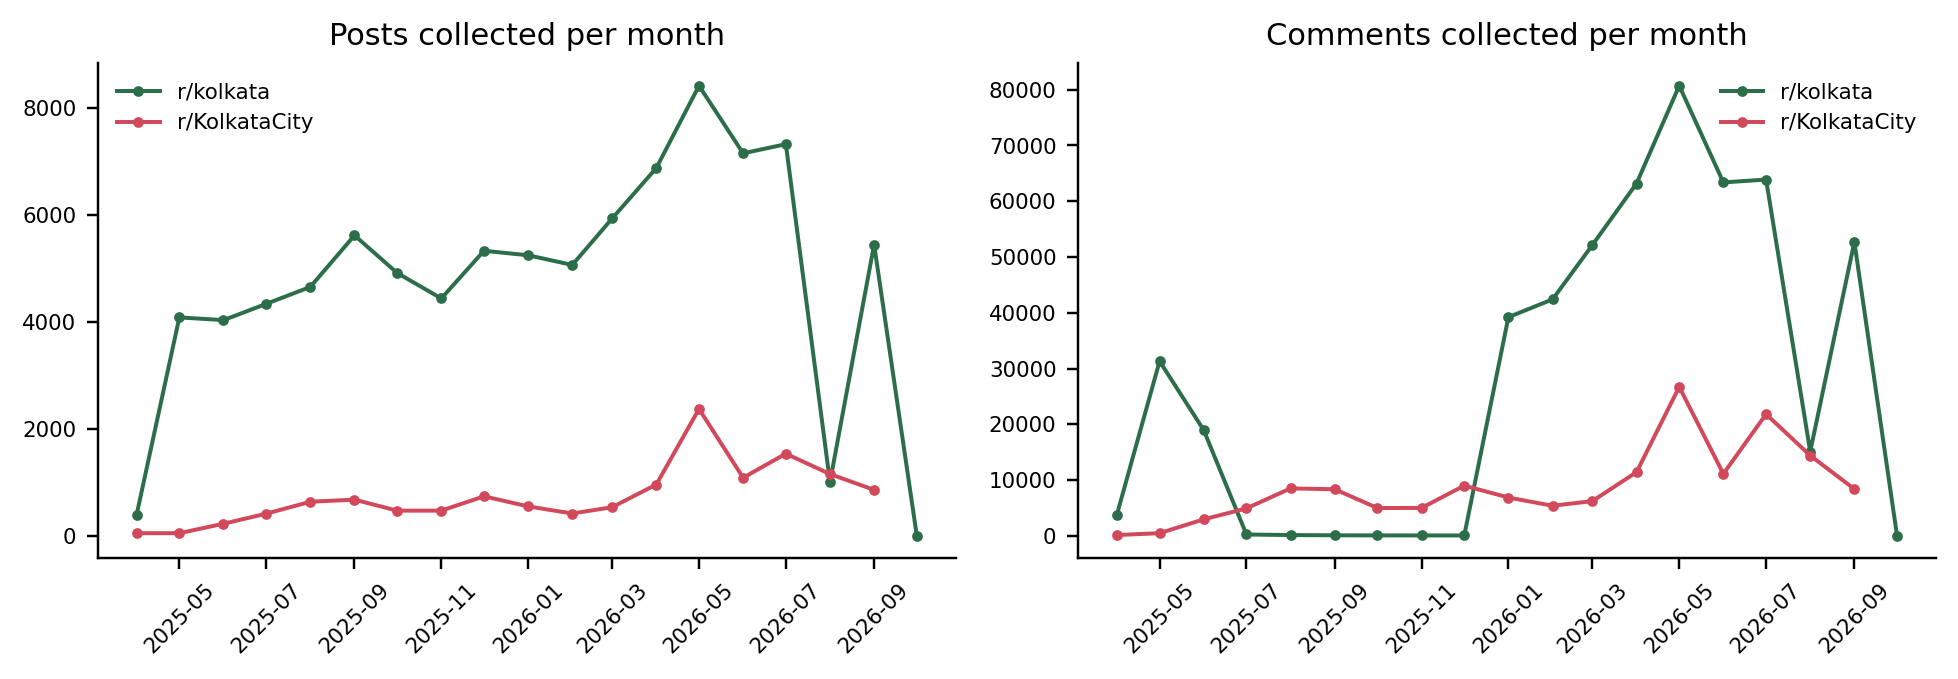
\includegraphics[width=0.95\textwidth]{monthly_activity_chart.png}
    \vspace{-0.3cm}
    \caption{\small Posts and comments collected per month for r/kolkata and r/KolkataCity. The
    mid-to-late-2025 dip in r/kolkata's comment counts is a deliberate, documented collection gap
    (Section~6.3), not a drop in subreddit activity.}
    \label{fig:chart}
\end{figure}
\vspace{-0.6cm}

\subsection{Discussion}
r/kolkata is, by every headline metric, substantially larger than r/KolkataCity — roughly 6.8
times as many posts and 3.2 times as many comments — despite both subreddits covering the same
collection window and being collected by the same pipeline. This size difference, discovered only
after collection was underway, is the direct cause of the comment-collection scope decision
discussed in Section~6.3. The near-zero count of duplicate post and comment IDs across the whole
dataset, together with zero duplicate IDs detected by validation, indicates that the
deduplication-by-Reddit-ID strategy (Section~4.6) is working as intended even across collection
runs that were interrupted and resumed multiple times.


% ---------------------------------------------------------------
% 6. CHALLENGES
% ---------------------------------------------------------------
\section{Challenges and Strategic Optimizations}

\subsection{Loss of the Originally Planned Data Source}
BrightData's Datasets API was the originally planned data source for this project, and it was the
source that supplied the project's first raw data: the earliest collection runs successfully
triggered and polled BrightData scraping jobs and wrote the resulting posts and comments to disk.
Continued reliance on it broke down for two separate reasons. First, BrightData's Datasets API is
metered, and the project's account was on a free/limited tier; the volume of posts and comments
needed for even a single subreddit-month of r/kolkata or r/KolkataCity exceeded that tier's
request allowance, so the account's usage limit was reached and further collection jobs could no
longer be triggered. Second, and independently of the quota issue, the development network began
intermittently blocking \texttt{api.brightdata.com}, raising a \texttt{SSLCertVerificationError}
(``self signed certificate in certificate chain'') — a signature consistent with local TLS
interception (VPN, proxy, or security software) rather than a code defect. Either failure alone
would have forced a change of data source; together, they made continuing to invest engineering
effort in BrightData clearly not worthwhile. Rather than paying to raise the account's quota and
simultaneously working around a network-level block, the pipeline was pivoted entirely to Arctic
Shift, a free, authentication-free archive unaffected by either failure mode, and the BrightData
client code was kept in place as inert legacy rather than deleted, in case the account or network
issue is later resolved.

\subsection{Unreliable Local Network During Long Unattended Runs}
The same TLS-interception signature that broke BrightData also intermittently affected Arctic
Shift requests, surfacing as connection resets, read timeouts, or transient
\texttt{422}/\texttt{503} responses. Empirically, retrying an identical failed request seconds
later typically succeeded, confirming these failures as transient rather than semantic (a
malformed request). This is handled by a six-attempt retry loop with backoff of \texttt{1, 2, 5,
15, 30, 60} seconds; only genuine non-retryable client errors propagate immediately. Two further
operational issues surfaced specifically during multi-hour unattended runs: the laptop going to
sleep silently stalled the collection process for however long it slept, fixed by wrapping long
runs in \texttt{caffeinate -i -s}; and a strictly sequential, one-post-at-a-time comment-collection
loop made throughput collapse whenever the backend was flaky, since every retry-laden post cost
whole minutes — fixed by shortening the initial backoff (transient errors usually recover in
about a second, not five) and by fetching several posts' comments concurrently via a thread pool
instead of one post at a time.

\subsection{An Unplanned Scope Decision: r/kolkata's True Size}
r/kolkata turned out to have approximately 91,000 posts over the collection window, versus
roughly 13,500 for r/KolkataCity — nearly seven times larger than the subreddit it was originally
expected to be comparable to. Comment-by-comment collection at that volume is a multi-day job
even with concurrency, and continuing to collect every month's comments in strict chronological
order would have delayed collection of the most recent, most immediately useful months. This was
resolved as a deliberate scope decision rather than a failure: comments for June 2025 through
December 2025 were never attempted for r/kolkata, while January 2026 through September 2026 (the
active range at the time) was prioritized and collected. Posts for the deferred months are fully
collected; only their comments are missing, and the gap is closed by a single, independently
re-runnable command (Section~6.5 of the project README) with no re-work of anything already done.

\subsection{Subreddit Metadata Fields With No Available Source}
Subreddit rules, the moderator list, pinned posts, and moderator announcements proved
unavailable from every source attempted: Reddit's own public \texttt{.json} endpoints return
HTTP 403 from this environment, and Arctic Shift's subreddit-metadata endpoint mirrors only the
subreddit's general "about" object (creation date, description, member count), not the separate
endpoints Reddit itself uses for rules, moderators, and announcements. Rather than approximating
these fields from indirect signals, each is recorded as \texttt{null} with an explanatory note,
so that a later consumer of the dataset can tell the difference between "this field was checked
and is genuinely unavailable" and "this field was never checked."

\subsection{Writing Very Large Processed Tables}
The processed comment table alone is approximately 226~MB and the post table approximately
74~MB, reflecting several hundred thousand records with free-text fields. Building these tables
by appending rows incrementally as raw data is processed, rather than materializing the entire
dataset in memory before writing, was necessary to keep processing within the memory limits of
the development machine, mirroring the same streaming-write discipline already used for the raw
JSONL caches.


% ---------------------------------------------------------------
% 7. FUTURE WORK
% ---------------------------------------------------------------
\section{Future Work}

As the project advances beyond the mid-term review, the following directions are planned:

\begin{itemize}
    \item \textbf{Close the Deferred Comment-Collection Gap:} Run the already-available comment
    collection command for r/kolkata, June 2025 through December 2025, to close the one
    deliberately deferred gap in an otherwise complete dataset (Section~6.3).

    \item \textbf{Close the Subreddit-Metadata Gap via OAuth:} Register a Reddit OAuth "script"
    application to obtain authenticated access to the rules, moderator-list, and pinned-post
    endpoints that are currently blocked on the unauthenticated public API, closing the one
    metadata gap identified in Section~6.4.

    \item \textbf{Deeper Comment Threads:} Investigate whether Arctic Shift's comment endpoint, or
    an alternative endpoint, can supply full parent-chain depth rather than the depth-1 cap
    currently imposed, to support analyses that require complete reply-thread structure.

    \item \textbf{Candidate Subreddit Expansion:} Use the originating subreddits recorded in
    \texttt{crossposts.csv} to identify and prioritize candidate communities for a future
    expansion of the pipeline beyond r/kolkata and r/KolkataCity, as anticipated by the original
    task brief.

    \item \textbf{Downstream Analysis:} With the collection and validation phase substantially
    complete, begin the actual computational social-science analysis the dataset was built to
    support — for example, topic or sentiment trends over time, or comparison of discussion
    patterns between the two subreddits' overlapping and non-overlapping user bases.

    \item \textbf{Runtime Benchmarking:} Quantify the wall-clock cost of the remaining comment
    backfill under the current concurrency settings, to decide whether a higher worker count is
    worth the corresponding increase in backend load.
\end{itemize}


% ---------------------------------------------------------------
% 8. CONCLUSION
% ---------------------------------------------------------------
\section{Conclusion}

This mid-term phase successfully built a resumable, parameterized pipeline that collects posts,
comments, subreddit metadata, and cross-post links for r/kolkata and r/KolkataCity from 1 April
2025 to the present, and converts this raw data into clean, de-duplicated processed tables
without ever needing to re-query either data source. The pipeline survived a complete loss of its
originally planned data source, BrightData — which supplied the project's initial raw data
before its account usage limit was reached and the development network began blocking it
outright — partway through the project, by pivoting to Arctic Shift as a free,
authentication-free alternative, and survived an unreliable local network
during multi-hour unattended runs through a combination of retry-with-backoff, sleep-prevention,
and concurrent comment fetching. As of this report, the dataset comprises 104,827 posts and
743,126 comments across both subreddits, with zero duplicate IDs and a fully documented, single
known gap: deferred comment collection for nine months of r/kolkata, itself a deliberate response
to that subreddit turning out to be nearly seven times larger than originally expected.

The month-level state-tracking design adopted in place of the literal date-range key sketched in
the original task brief (Section~4.5) is the central engineering decision of this phase, and the
fact that every API call logged in \texttt{collection\_log.csv} corresponds to genuinely
uncollected data, with no redundant re-fetching observed across repeated interrupted-and-resumed
runs, is the strongest evidence that this decision was the right one. The immediate next steps
are to close the one remaining comment-collection gap, obtain OAuth access to close the subreddit
rules/moderator-metadata gap, and begin the downstream analysis this collection phase was built
to support, as outlined in Section~7.

Beyond the specific numbers, this phase demonstrates that a complete, multi-source, resumable
data-collection pipeline — from raw third-party API responses, through incremental caching and
state tracking, to validated processed tables — can be built and operated reliably within the
computational and networking constraints of a course project, provided the operational failure
modes documented in Section~6 are designed around deliberately rather than discovered too late
to recover from.


% ---------------------------------------------------------------
% 9. APPENDIX
% ---------------------------------------------------------------
\section{Appendix}

\subsection*{A.1 User Overlap Between Subreddits}
Table~\ref{tab:overlap} reports the user-overlap breakdown computed from \texttt{users.csv},
as required by the task brief's user-participation specification.

\begin{table}[h]
\centering
\small
\caption{User overlap between r/kolkata and r/KolkataCity.}
\label{tab:overlap}
\begin{tabular}{lr}
\toprule
\textbf{Category} & \textbf{Users} \\
\midrule
Total unique users (either subreddit) & 98{,}855 \\
Users active in both subreddits & 11{,}836 \\
Users active only in r/kolkata & 60{,}047 \\
Users active only in r/KolkataCity & 26{,}972 \\
\bottomrule
\end{tabular}
\end{table}

\subsection*{A.2 Reproduction Environment and Configuration}
Table~\ref{tab:env} summarizes the software environment and key configuration settings used to
produce the dataset reported above.

\begin{table}[h]
\centering
\caption{Software environment and configuration settings.}
\label{tab:env}
\begin{tabular}{@{}lp{9cm}@{}}
\toprule
\textbf{Setting} & \textbf{Value} \\
\midrule
Active data source & Arctic Shift (\texttt{--source arcticshift}) \\
Legacy data source & BrightData Datasets API v3 (used for initial raw data; retired after the
account's request quota was reached and TLS-interception errors began blocking it) \\
Collection window & 2025-04-01 through present, monthly chunks \\
Comment-fetch concurrency & 5 workers (default), \texttt{ThreadPoolExecutor} \\
Retry policy & 6 attempts, backoff 1/2/5/15/30/60 seconds \\
Comment tree depth & 2 levels (top-level + direct reply) \\
State-tracking granularity & \texttt{(subreddit, data\_type, month)} \\
Core libraries & Python 3, \texttt{requests}, \texttt{pandas}, \texttt{NumPy} \\
\bottomrule
\end{tabular}
\end{table}

\subsection*{A.3 Repository and Output Artifacts}
The pipeline described in this report is organized into four top-level directories under
\texttt{reddit\_kolkata/}: \texttt{raw/}, containing cached JSONL API responses partitioned by
subreddit and month; \texttt{processed/}, containing the five derived CSV tables
(\texttt{posts.csv}, \texttt{comments.csv}, \texttt{crossposts.csv}, \texttt{users.csv},
\texttt{monthly\_activity.csv}) and \texttt{validation\_report.json}; \texttt{subreddit\_metadata/},
containing one dated JSON snapshot per metadata-collection run; and \texttt{collection\_code/},
containing every collection, processing, and validation script. Two ledger files,
\texttt{collection\_state.csv} and \texttt{collection\_log.csv}, sit at the top level and are
consulted before every API call, as described in Section~4.5.

% ---------------------------------------------------------------
% 10. REFERENCES
% ---------------------------------------------------------------
\section{References}

\begin{enumerate}
    \item Baumgartner, J., Zannettou, S., Keegan, B., Squire, M., \& Blackburn, J. (2020).
    \textit{The Pushshift Reddit Dataset}. Proceedings of the International AAAI Conference on
    Web and Social Media (ICWSM), 14, 830--839.

    \item Heitmann, A. \textit{Arctic Shift: A Continuously Updated Archive of Reddit Content}.
    GitHub repository. \url{https://github.com/ArthurHeitmann/arctic_shift}

    \item BrightData. \textit{Datasets API: Trigger a Collection or Discovery}. \\
    \small\url{https://docs.brightdata.com/api-reference/marketplace-dataset-api/trigger-a-collection-or-discovery}\normalsize

    \item Reddit, Inc. \textit{Reddit API Documentation}. \url{https://www.reddit.com/dev/api/}

    \item McKinney, W. (2010). \textit{Data Structures for Statistical Computing in Python}.
    Proceedings of the 9th Python in Science Conference (SciPy), 56--61.

    \item Harris, C. R., Millman, K. J., van der Walt, S. J., Gommers, R., Virtanen, P.,
    Cournapeau, D., et al. (2020). \textit{Array Programming with NumPy}. Nature, 585,
    357--362.

    \item Nygard, M. T. (2018). \textit{Release It!: Design and Deploy Production-Ready
    Software} (2nd ed.). Pragmatic Bookshelf. (Retry-with-backoff and stability-pattern
    reference for the resumable-collection design in Section~4.)
\end{enumerate}

\end{document}
